% Círculo trigonométrico (ângulos em radianos)
% Feito para o ÉguaTeX (eguatex.com.br). Uso livre (CC0 1.0).
%
% Compile e pronto: sai só a figura, em PDF.
% Para pôr no seu trabalho, use o PDF com \includegraphics ou copie
% o bloco tikzpicture para dentro de uma figure.
\documentclass[tikz,border=4pt]{standalone}
\usepackage[T1]{fontenc}
\usepackage{lmodern}
\usepackage{amsmath}

\colorlet{corSen}{red!75!black}
\colorlet{corCos}{blue!75!black}
\colorlet{corTg}{green!45!black}

\begin{document}
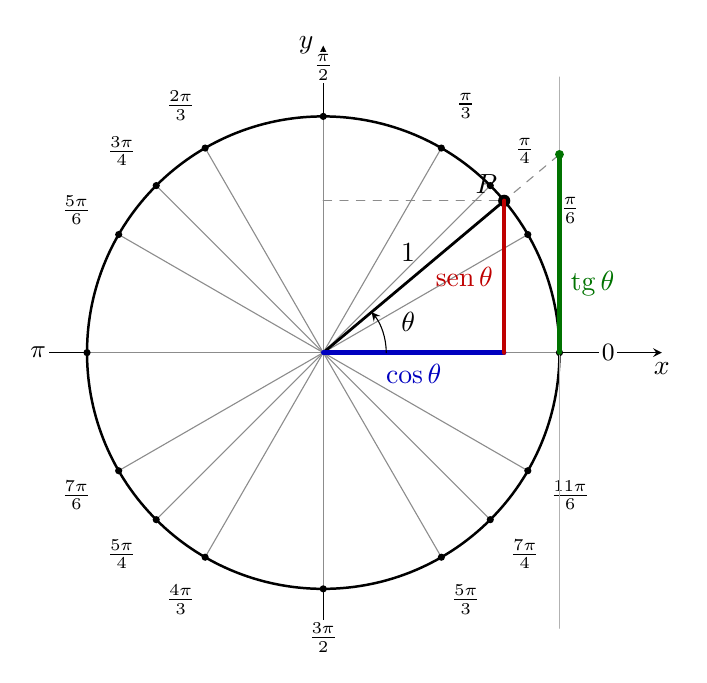
\begin{tikzpicture}[line cap=round, line join=round, >=stealth]

% Mude estes números e o desenho e os rótulos acompanham.
\def\R{3}      % raio do círculo, em cm
\def\ang{40}   % ângulo destacado, em graus (entre 5 e 80 para a tangente caber)

\pgfmathsetmacro{\c}{\R*cos(\ang)}
\pgfmathsetmacro{\s}{\R*sin(\ang)}
\pgfmathsetmacro{\t}{\R*tan(\ang)}

% eixos e círculo
\draw[->] (-\R-0.7,0) -- (\R+1.3,0) node[below] {$x$};
\draw[->] (0,-\R-0.7) -- (0,\R+0.9) node[left] {$y$};
\draw[line width=0.9pt] (0,0) circle[radius=\R];

% ângulos notáveis: tracinho no círculo e valor por fora
\foreach \a/\rot in {0/0, 30/\frac{\pi}{6}, 45/\frac{\pi}{4}, 60/\frac{\pi}{3}, 90/\frac{\pi}{2},
    120/\frac{2\pi}{3}, 135/\frac{3\pi}{4}, 150/\frac{5\pi}{6}, 180/\pi, 210/\frac{7\pi}{6},
    225/\frac{5\pi}{4}, 240/\frac{4\pi}{3}, 270/\frac{3\pi}{2}, 300/\frac{5\pi}{3}, 315/\frac{7\pi}{4}, 330/\frac{11\pi}{6}} {
  \draw[black!45] (0,0) -- (\a:\R);
  \fill (\a:\R) circle[radius=1.3pt];
  \node[font=\small, fill=white, inner sep=1pt] at (\a:\R+0.62) {$\rot$};
}

% reta tangente ao círculo em (R, 0)
\draw[black!30] (\R,-\R-0.5) -- (\R,\R+0.5);

% raio até o ponto P e prolongamento até a tangente
\draw[black!45, dashed] (0,0) -- (\R,\t);
\draw[line width=1pt] (0,0) -- (\ang:\R) node[pos=0.55, above left=-1pt] {$1$};
\fill (\ang:\R) circle[radius=2.2pt];
\node[above left=-1pt] at (\ang:\R) {$P$};

% projeções: cosseno, seno e tangente
\draw[corCos, line width=1.6pt] (0,0) -- (\c,0) node[midway, below] {$\cos\theta$};
\draw[corSen, line width=1.6pt] (\c,0) -- (\c,\s) node[midway, left] {$\operatorname{sen}\theta$};
\draw[black!45, dashed] (0,\s) -- (\c,\s);
\draw[corTg, line width=1.6pt] (\R,0) -- (\R,\t) node[pos=0.35, right] {$\operatorname{tg}\theta$};
\fill[corTg] (\R,\t) circle[radius=1.6pt];

% ângulo theta
\draw[->] (0.8,0) arc[start angle=0, end angle=\ang, radius=0.8];
\node at ({\ang/2}:1.15) {$\theta$};
\end{tikzpicture}
\end{document}
